\section{Multi-Processor Scheduling \weekDoran{5}}
	\subsection{Amdahls Law}
		Amdahls Law	describes the potential possible speed up, if a part of the code is parallelized by using a multi processor system.
		\begin{longtable}{p{0.6\linewidth}p{0.35\linewidth}}
			\vspace{0pt}
			
			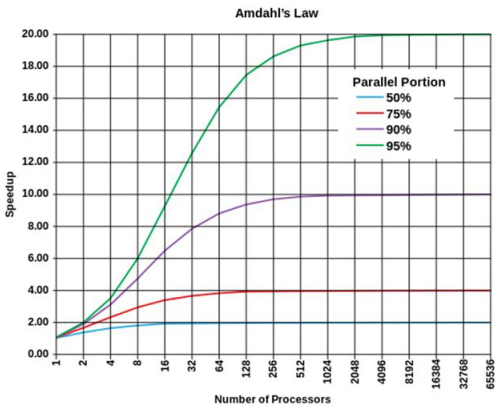
\includegraphics[width=0.6\textwidth]{./pictures/amdahl.png}
			&
			\begin{equation*}
				\begin{aligned}
					S(n) &= \frac{1}{1-p-\frac{p}{n}} \\
					S(n) &\leq  \frac{1}{1-p} \\
					S &= \text{Speedup} \\
					p &= \text{Parallel Portion} \\
					n &= \text{Number of Processors} \\
					S(n) &= \frac{T}{t_s+\frac{t_p}{n}} \\
					S(n) &\leq  \frac{T}{T-t_p}=\frac{T}{t_s} \\
					T &= \text{Total execution time} \\
					t_p &= \text{Parallel execution time} \\
					t_s &= \text{Serial execution time} \\
				\end{aligned}
			\end{equation*}
		\end{longtable}

	\subsection{TAS (Test and Set) and TTAS (Test and Test and Set)}
		\textbf{TAS:} Atomic instruction, noninterruptible; slow because of bus locking and cache invalidation \\
		\textbf{TTAS:} Only calls TAS when it is not already locked\\
		\textbf{Example:} Each thread has it's own cache. Cache is updated only when the variable is marked as dirty. TAS (at the OS level) marks the variable as dirty whenever it's called, regardless of whether it succeeded in setting the value or not. This is what causes a big overhead. Because of that, all threads keep invalidating the cache all the time. In TTAS case, you avoid calling TAS as much and therefore only invalidate cache on, now much rarer, TAS calls and when you release the lock.
		
	\subsection{Scheduling}
		\begin{longtable}{|>{\bfseries}p{0.1\linewidth}|p{0.45\linewidth}|p{0.4\linewidth}|}
			\hline
			SQMS
			&
				\begin{compactitem}
					\item Single Queue Multiprocessor Scheduling
					\item With a simple task queue and no special arrangements, the schedule such as the middle picture will happen
					\item Every time a task is swapped to another CPU the cache has to be reloaded.
				\end{compactitem}
			&
			\vspace{0pt}
			
			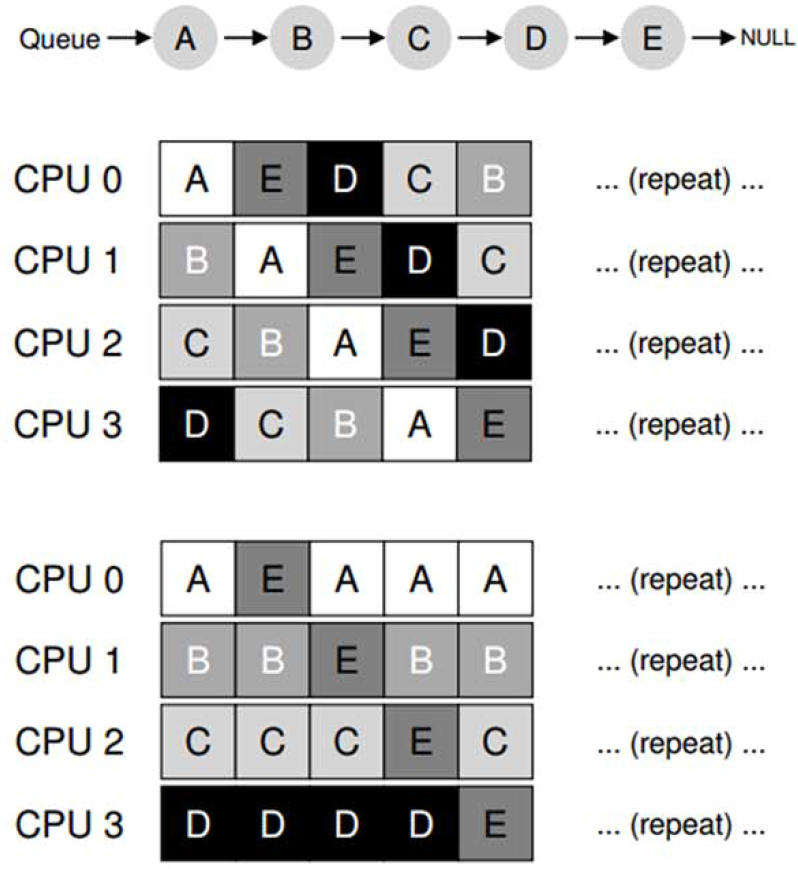
\includegraphics[width=\linewidth]{./pictures/sqms.png} \\
			\hline
			MQMS
			&
			\begin{compactitem}
				\item Multi Queue Multiprocessor Scheduling
				\item Scales better as lock and cache contention prevented and cache affinity provided
				\item Suffers from load-imbalancing $\rightarrow$ A gets too much processing time, whereas B and D have to share. If A stops then B and D still share the same CPU and CPU 0 is idle.
			\end{compactitem}
			&
			\vspace{0pt}
			
			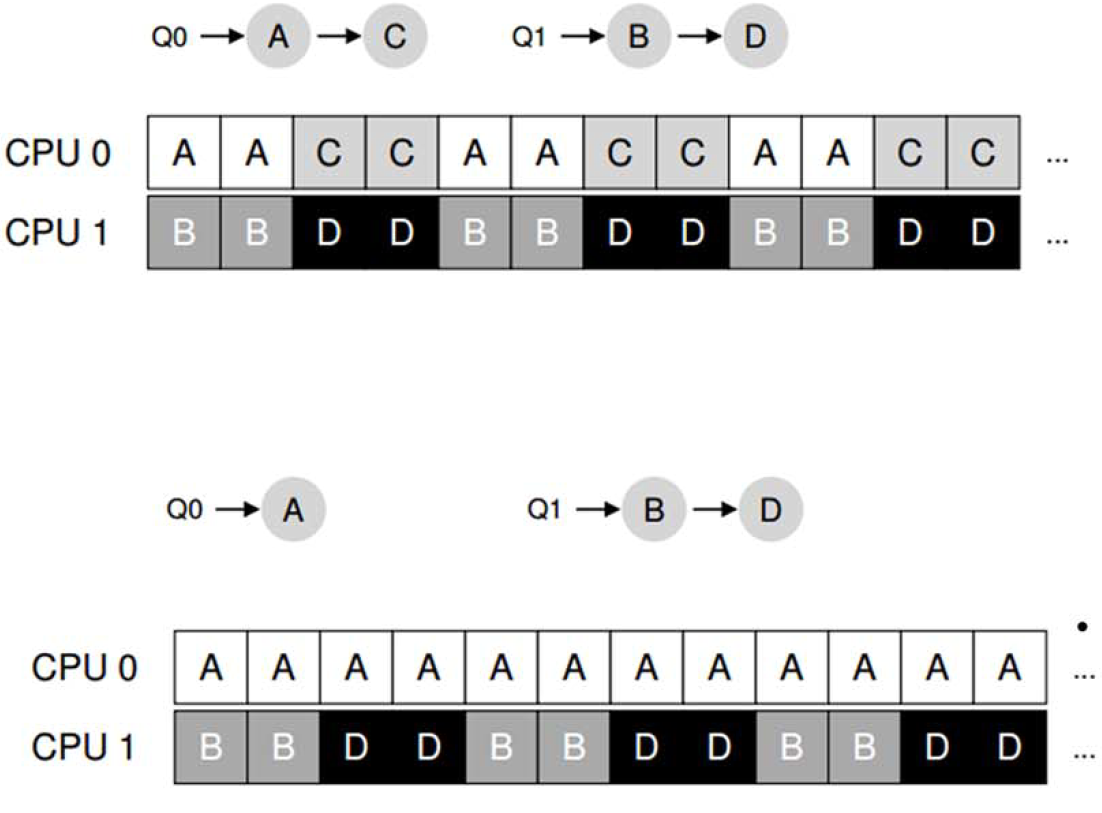
\includegraphics[width=\linewidth]{./pictures/mqms.png}\\
			\hline
			Continuous migration \newline\newline
			Work stealing
			&
			\begin{compactitem}
				\item Continuous migration: Cache affinity is partially kept
				\item Work stealing: A queue will look at other queues to see if they have more tasks and takes them if they do
			\end{compactitem}
			&
			\vspace{0pt}
			
			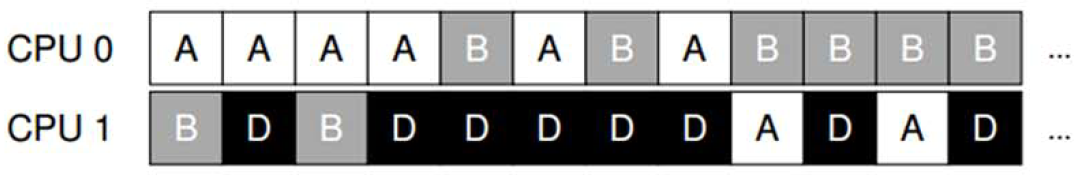
\includegraphics[width=\linewidth]{./pictures/mqms2.png}\\
			\hline
		\end{longtable}
	
	\subsection{Network on Chip}
		There are three essential types of on-chip communication systems: Point to Point (P2P, a), Bus Systems (b) and Network on Chip (c). \\
		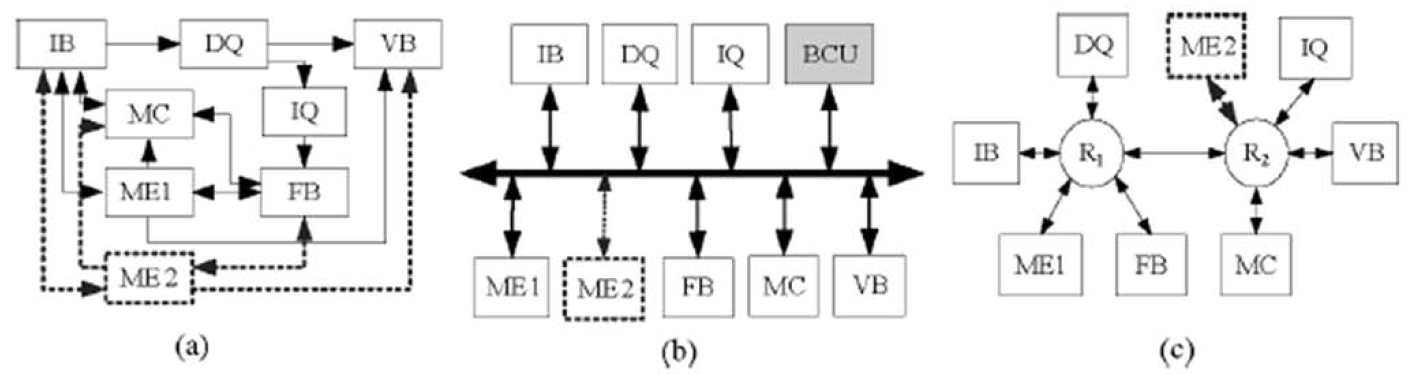
\includegraphics[width=\linewidth]{./pictures/network.png}\\
		NOC offers high bandwidth and scaleability.